The following image represents the deployment diagram of the SafeStreets architecture. It shows the logical division of the software architecture as well as the distribution of the software components to their target nodes, on which they will be deployed.

\begin{figure}[H]
  \centering
  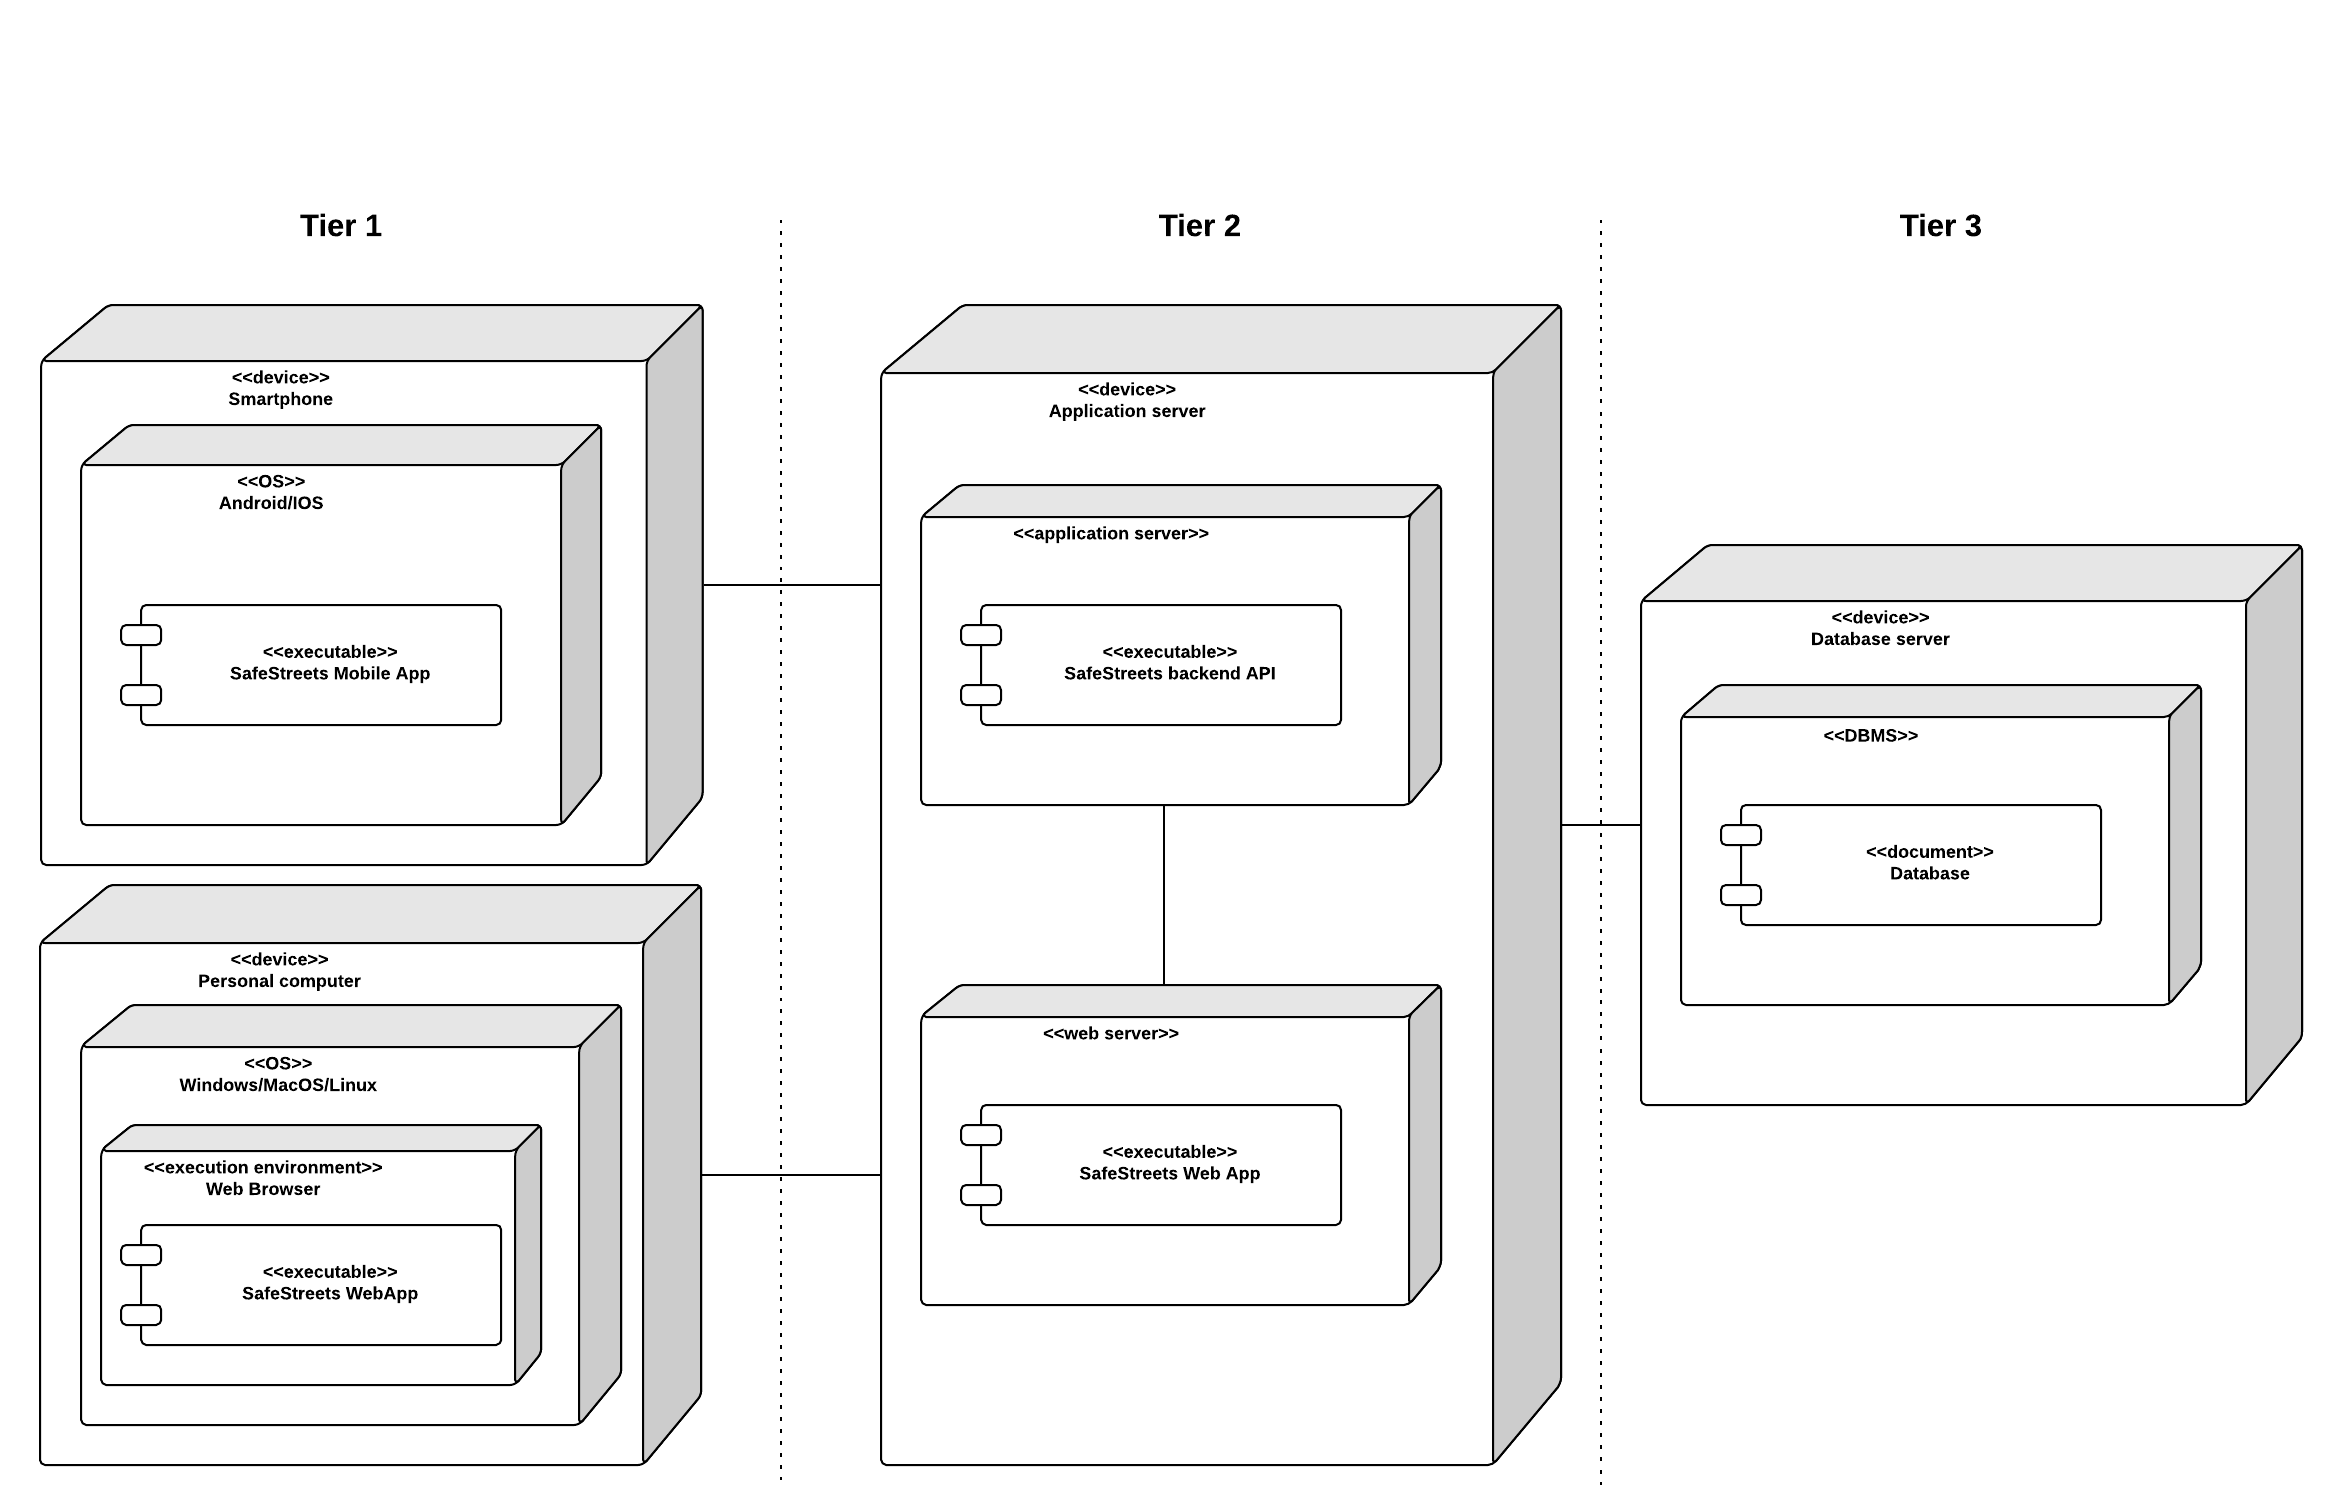
\includegraphics[width=1\textwidth]{Deployment_Diagram}
  \caption{Deployment diagram}
  \label{fig:deployment_diag}
\end{figure}

The diagram represent the architectural pattern chose for the deployment of the SafeStreets service. It's a three tier architecture that has been conceived in order to provide a fast and lightweight client for both the users and the authorities. 
It is also important to note that the previous diagram is focused only on those components that will have to be effectively developed,that's why, for example, the maps and the plate recognitions services are not displayed in the diagram, as they already exist.
Here is a short explanation of what each tier does:
\begin{itemize}
  \item \textbf{Tier 1}: The first tier is the presentation tier of the architecture. The main function of this layer is to host the  the application of the users and the Web app of the authorities. It is worth noting that there's little or nothing business logic present in this layer apart from those that are strictly required for the correct functioning of the applications; the application and the Web App are only presentation client that will have to interact with the second tier in order to get/elaborate information. As for the deployment aspect: the mobile application must be developed in order to cover the most of the devices, so it must be runnable at least on Android and IOS (to reduce the development time one could also think to use a cross-platform development framework) while the Web app must be compatible with the most modern web browser such as: Edge, Chrome, Firefox and Safari. As stated before the applications in this tier are just thin clients so they need to interact with the application server in order to get information. The Mobile application asks the information directly to the application server via the backend API while the Web app communicate with the web server that will eventually ask to the application server for data. All the communications are performed with RESTful calls over a secure connection;
  % TODO: check tier 2
  \item \textbf{Tier 2}: The second tier of the architecture is called the logic layer, it is the place in which all the business logic is located; all the functionalities and the elaborations are computed here. The implementation is achieved via a server that runs two subservices separately: the Application server and the Web server. The Application server hosts the core of the system that is to say the SafeStreets Backend API, this is the piece of software that will handle all of the requests and the offered services. Instead the Web server hosts the content for the web app, in case that some page needs to be created with some data, the Web server can communicate with the backend API in order to retrieve the information needed;
  \item \textbf{Tier 3}: The final layer is the Data tier. It handles the data access with the remote NoSQL database. The    choice to move this into a separate tier is due to the fact       that with this approach the data are independent from the         business logic.
  % TODO: Finish with motivation of NoSQL database
\end{itemize}
